\documentclass[12pt,a4paper]{article}
\usepackage[utf8]{inputenc}
\usepackage{amsmath}
\usepackage{amsfonts}
\usepackage{amssymb}
\usepackage{graphicx}
\usepackage{subcaption}
\usepackage{float}
\usepackage{multirow}
\usepackage{rotating}

\author{Team Gamma \\ {\small Ajda Frankovič, Martin Preradović, Niki Bizjak}}
\title{Face recognition}
\date{}
\begin{document}
    \maketitle

    In our third homework we were training a classifier to recognize 21 different faces.

    \section{Preparing training and testing data}

    \subsection{Obtaining images}

    This time we needed images of faces under different conditions. We took about 30 photos of each prined face. % and about x photos of each face in gazebo
    One set of images of printed faces was taken from 1m, 1.5m and 2m of distance under different viewing angles (0°, 30°, 45°) in the daylight. We also took some photos at 60°viewing angle and distance of 1m.
    The other set of images of printed faces was taken form 1m distance at different viewing angles and under two levels of lower light.
    For consistency, we tried to take images in a way that the face is in the center of the image.
    % gazebo images description
    In total, we obtained around XY images of faces. % ~630 printed + ? gazebo

    Below we present a subset of our data.

    \begin{figure}[H]
        \centering
        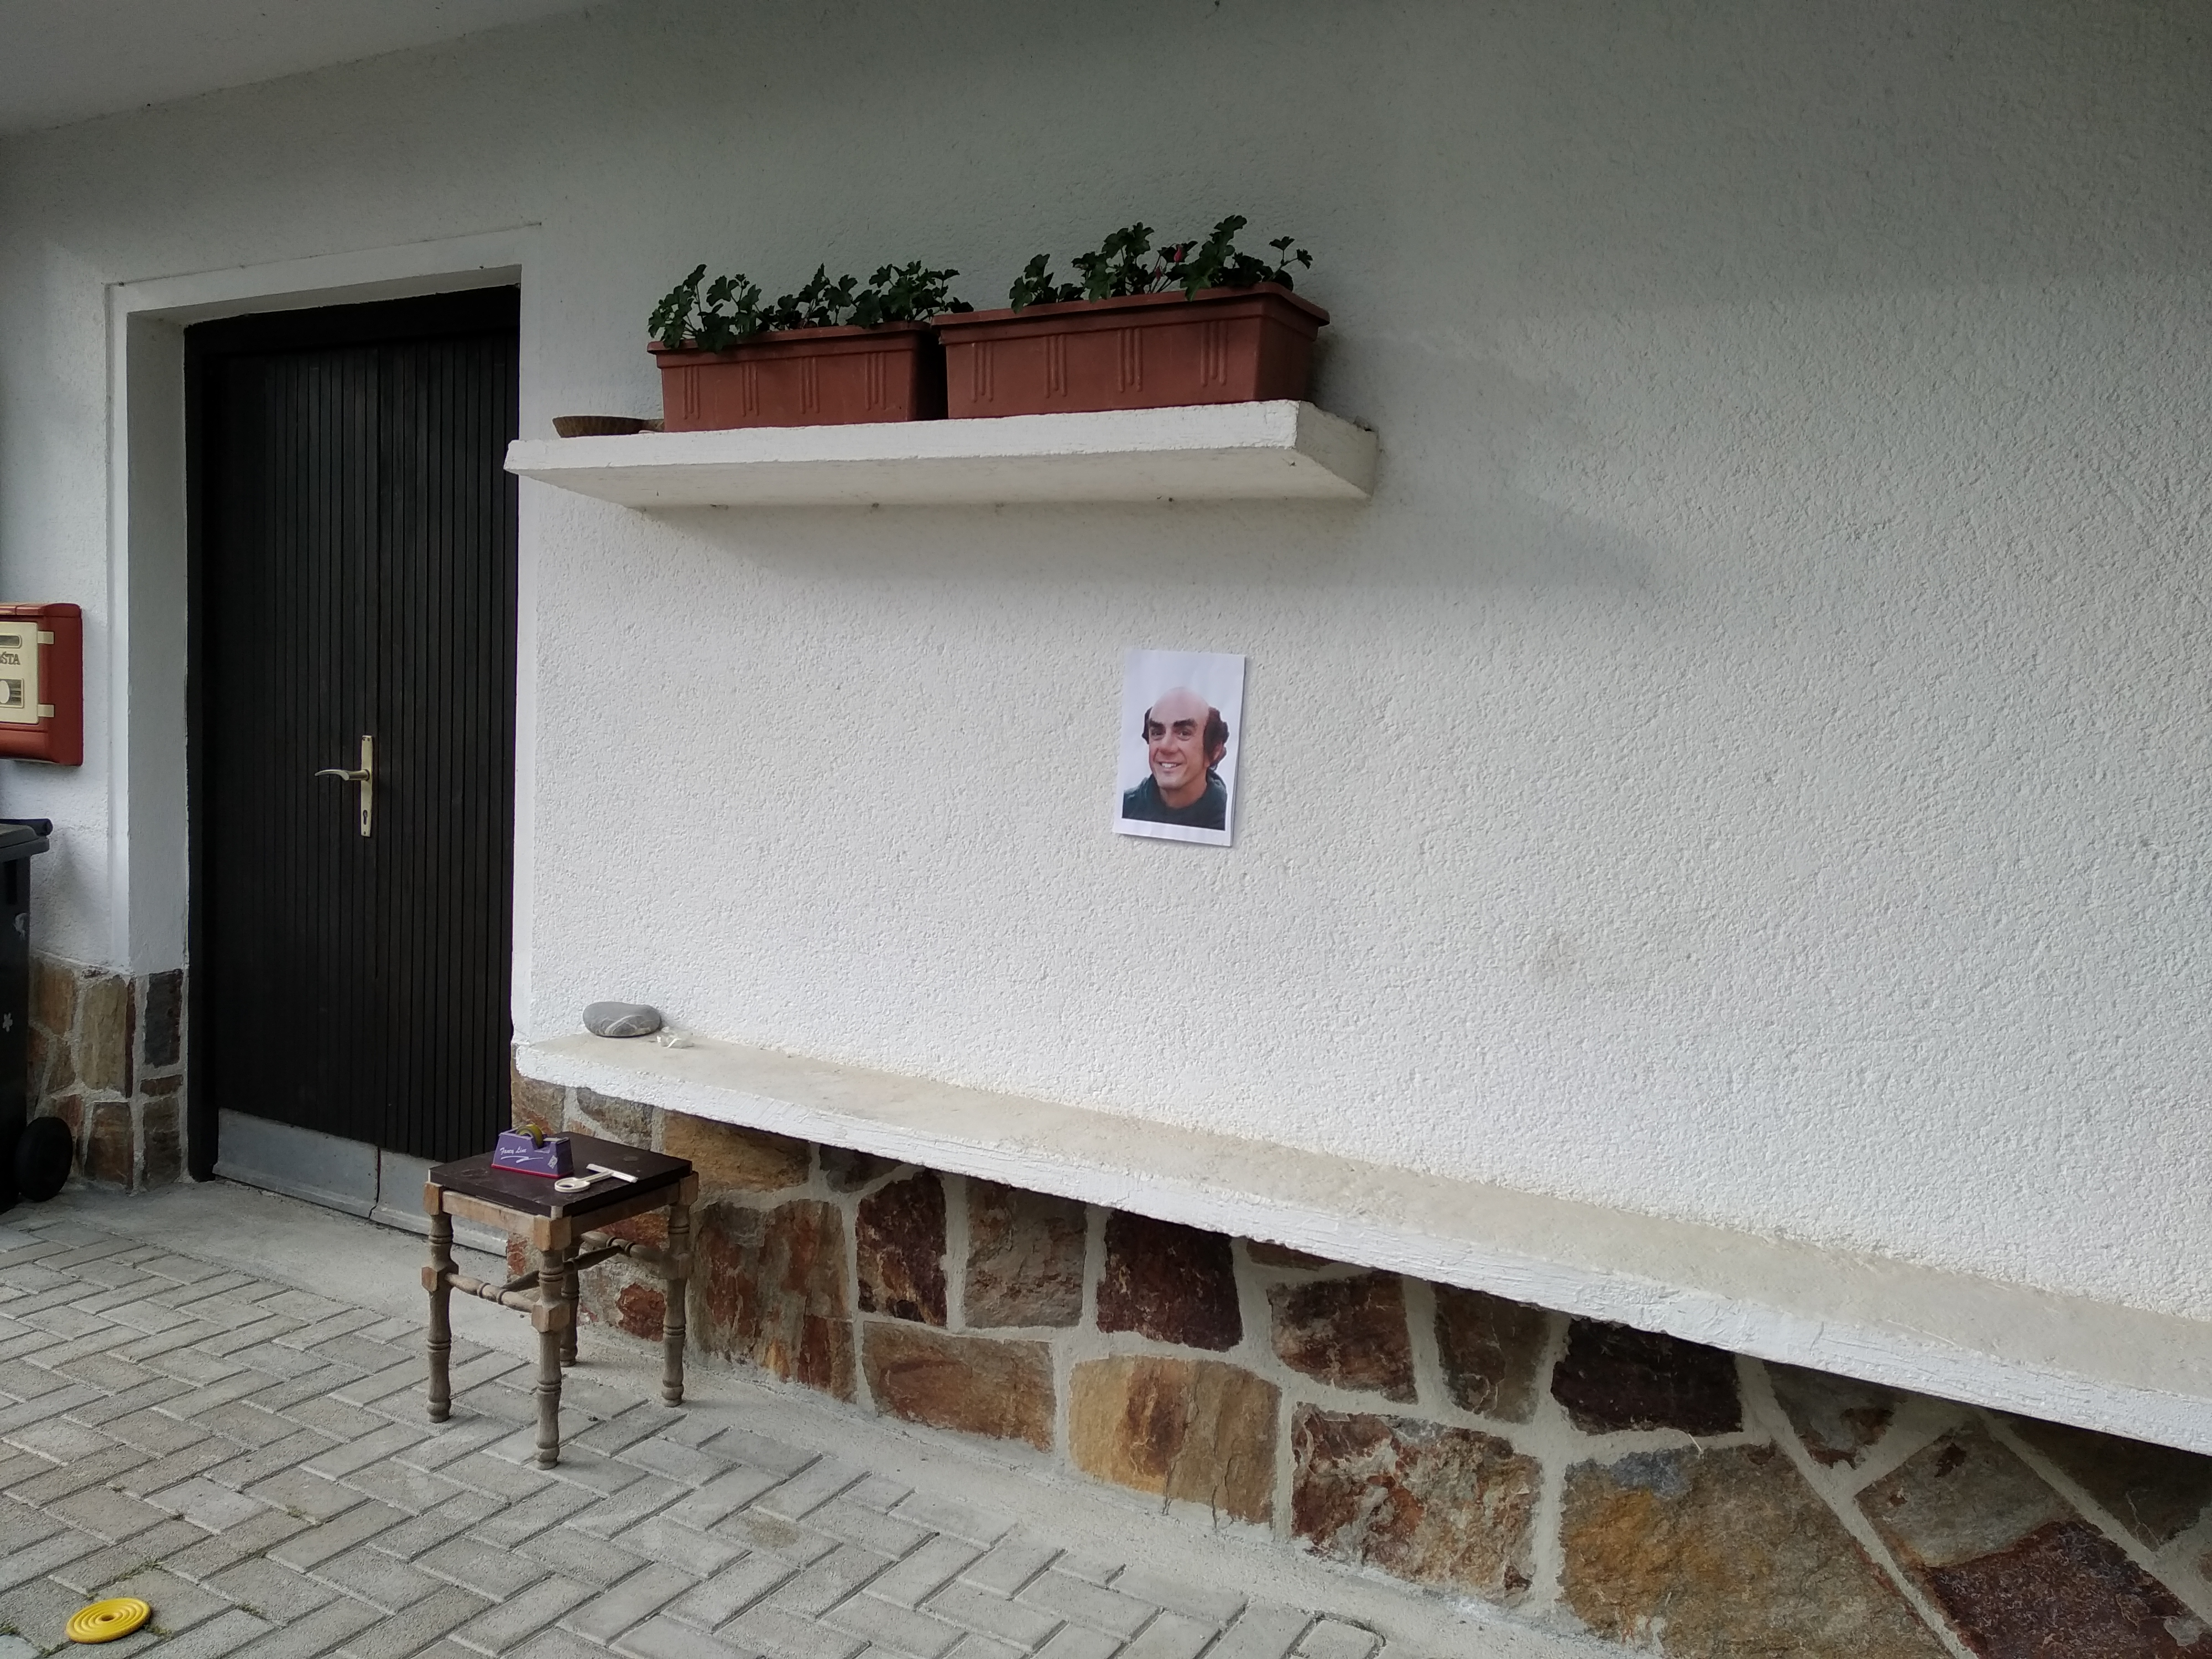
\includegraphics[width=.20\linewidth]{images/gargamel_outside_30_2m.jpg}
        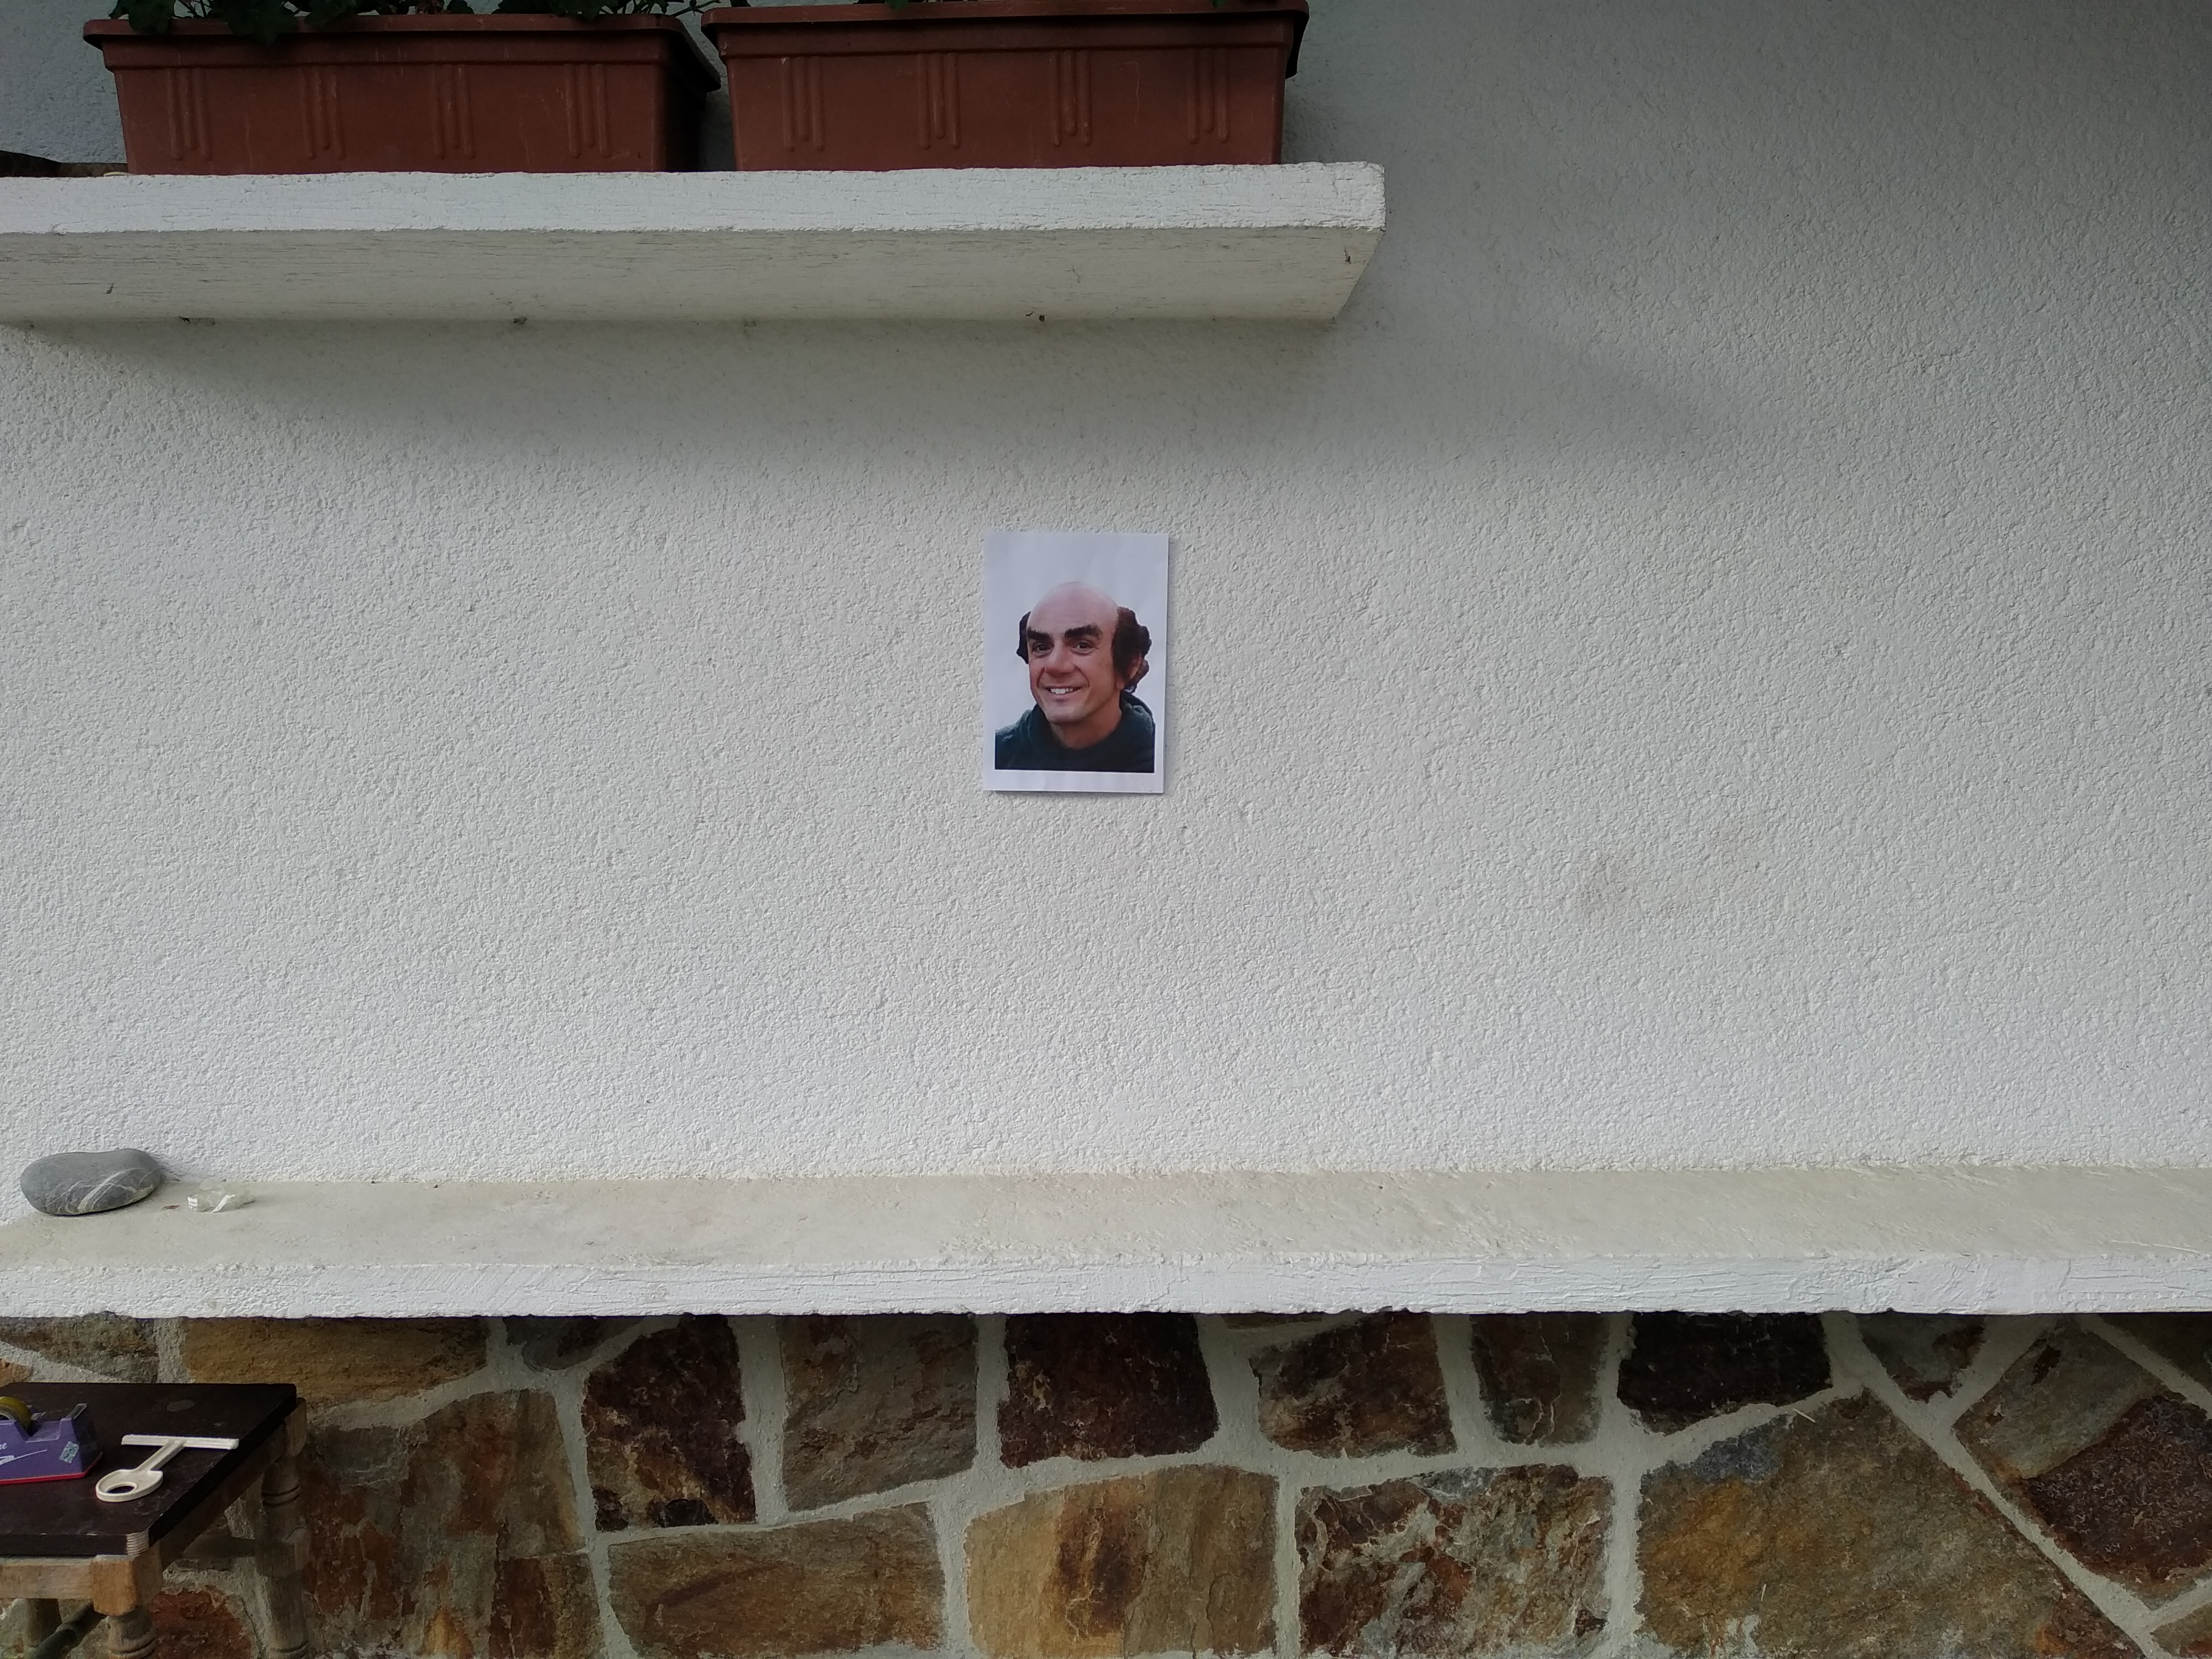
\includegraphics[width=.20\linewidth]{images/gargamel_outside_0_15m.jpg}
        \includegraphics[width=.20\linewidth]{images/gargamel_inside_30_light.jpg}
        \includegraphics[width=.20\linewidth]{images/gargamel_inside_30_dark.jpg}
        \caption{Photos of faces}
    \end{figure}

    \subsection{Dividing images into training and testing set}

    We divided our images in two sets. % how we did that

    \section{Training the classifier}

    \subsection{Preprocessing data}

    % resizing, cropping, detecting faces

    \subsection{Choosing a classifier}

    % what we chose/tried, why we thought this was a good idea. How it works.

    \section{Analysing the results}

    % accuracy of all tested classifiers, confusion matrix for the best classifier, 
    % discussion on which hypotesis in "Choosing a calssifier" turned out to be true and which didn't. Why the accuracy isn't 100%? What will we use for our robot?

\end{document}